%!TEX root = emnlp2016.tex

In this section we develop the Capsule model for detecting and characterizing events.  Capsule relies on text data sent between entities over time, and builds on topics models. We first give the intuition on Capsule, then review topic models at a high level and formally specify the model.  We also describe how to explore a corpus using Capsule, discuss Capsule's relationship to Poisson processes, and describe how we learn its hidden variables.

\begin{figure}
\centering
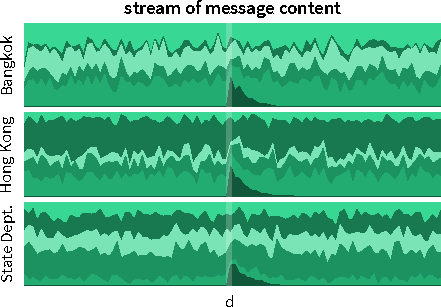
\includegraphics[width=\linewidth]{fig/cartoon.pdf}
\caption{Cartoon intuition of Capsule; the $y$ axis is the stacked proportion of messages about various subjects during a given time interval.  The Bangkok embassy, Honk Kong embassy, and State Department all have typical concerns about which they usually send messages.  When an events occurs at time $t$, the stream of message content alters to include the event, then fades back to ``business as usual.''  Capsule discovers both entities' typical concerns and the event locations and content.}
\label{fig:cartoon}
\end{figure}

Consider an entity like the Bangkok American embassy, shown in Figure~\ref{fig:cartoon}.  We can imagine that there is a stream of messages (or \emph{diplomatic cables}) being sent by this embassy---some might be sent to the US State Department, others to another American embassy like Hong Kong.  An entity will usually talk about certain topics; the Bangkok embassy, for instance, is concerned with topics regarding southeast Asia more generally.

Now imagine that at a particular time $t$, an event occurs, such as the capture of Saigon during the Vietnam war.  We do not directly observe that events occur, but we do observe the message stream.  Using this stream, each event be described as a distribution over the vocabulary, similar to how topics are distributions over these same terms.  When an event occurs, the message content changes for multiple entities. The day following the capture of Saigon, the majority of the diplomatic cables sent by the Bangkok embassy were about Vietnam war refugees.
Thus we imagine that an entity's stream of messages is controlled by what it usually talks about as well as the higher level stream of unobserved events.

\parhead{Background: Topic Models.} Capsule builds on topic models.  Topic models are algorithms for discovering the main themes in a large collection of documents; each document can then be summarized in terms of the global themes.  More formally, a topic $k$ is a probability distribution over the set of vocabulary words.  Each document $d$ is represented as a distribution over topics $\theta_d$.  Thus we can imagine that when we generate a document, we first pick which topics are relevant (and in what proportions).  Under the LDA topic model~\cite{Blei:2003}, we know the number of words in each document.  Then, for each word, we select a single topic from this distribution over topics, and finally select a vocabulary term from the corresponding topic's distribution over the vocabulary.  Alternatively, we can cast topic modeling as factorization, such as in Poisson factorization~\cite{Gopalan:2014b}, and draw a word count for each term in the vocabulary.

Topic models are often applied to provide a structure for an otherwise unstructured collection of documents.  Documents, however, are often accompanied by metadata, such as the date written or author attribution; this information is not exploited by traditional topic models.  The Capsule model uses both author and date information to identify and characterize events that influence the content of the collection.

\parhead{Model Specification.}
We formally describe Capsule. The observed data are word counts $w_{d,v}$ for document $d$ and vocabulary term $v$; each document $d$ also has an author (or entity) $a_d$ and a time (or date) interval $i_d$ associated with it.

The hidden variables of this model are general topics of conversation $\beta$, authors' typical concerns $\phi$, event descriptions $\pi$, event strengths $\psi$, and document-specific topics $\theta$ and event relevancy $\epsilon$.  %The graphical model in Figure~\ref{fig:graphicalmodel} shows considers dependencies between these latent parameters and the observed data.

% \begin{figure}[htb]
% \centering
% 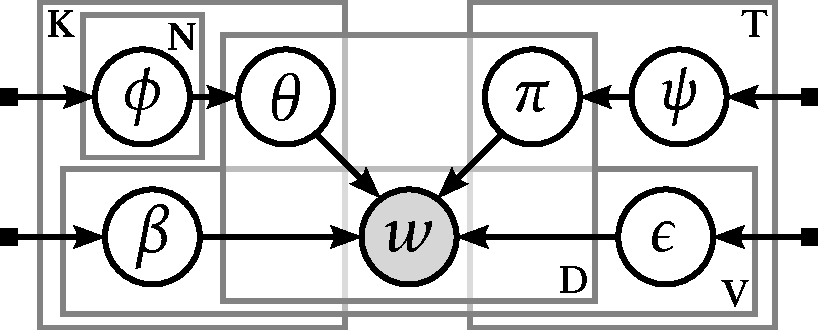
\includegraphics[width=\linewidth]{fig/graphicalmodel.pdf}
% \caption{A directed graphical model of Capsule to show considered dependencies. Shaded nodes $w$ are observed word counts.  Unshaded nodes are hidden variables---at the global level, these are topics $\beta$, entity typical concerns $\phi$, interval strength $\epsilon$, and interval content descriptions $\pi$.  At the document level, we have hidden variables for local entity concerns $\theta$ and interval relevancy $\epsilon$. Plates denote replication: there are $D$ documents, $T$ intervals, $N$ entities, $K$ topics, and $V$ vocabulary terms. Fixed hyperparameters are indicated by black squares.}
% \label{fig:graphicalmodel}
% \end{figure}

As in topic modeling, we represent the general topics of conversation with a $K\times V$ matrix $\beta$, where $K$ is a low dimensional number of topics that we wish to capture, and $V$ is the size of our vocabulary; each row $\beta_k$ is normalized such that it represents the probability of seeing vocabulary word $v$ when discussing topic $k$.  As a generative process, we draw these general topics from a Dirichlet distribution, or $\beta_k \sim \mbox{Dirichlet}_V (\alpha_\beta).$ 

In addition to using these general topics to represent entity concerns, each entity $n$ has its own exclusive topic $\beta^{(n)}_{0}$, which can be appended as a bias row to the general topics $\beta$.  These entity-specific topics are drawn from a Dirichlet, just as the general topics, and are similar to
background topics~\cite{paul2012model}.  Without these entity topics, entity-specific stop words (e.g. ``Parisian'' for the Paris embassy) would dominate the general topics.

The concerns of author $n$ are represented with $\phi_n$, a $(K+1)$-dimensional topic vector, where each element is drawn from a gamma distribution, or $\phi_{n,k} \sim \mbox{Gamma}(s_\phi, r_\phi),$\footnote{We use the shape-rate parameterization for all Gamma distributions.} and the first element of the concern vector $\phi_{n,0}$ describes how much the entity $n$ relies on its exclusive topic $\beta^{(n)}_0$

Similar to topic modeling, we represent the contents of each document in topic space; each document $d$ has a $(K+1)$-dimensional latent parameter $\theta_d$ to describe the particular contents of that document.  Unlike traditional topic models, each document $d$'s topics depend on the concerns of the author $a_d$; each document topic $\theta_{d,k}$ is drawn from a gamma distribution parameterized by the corresponding author concerns $\phi_{a_d,k}$: $\theta_{d,k} \sim \mbox{Gamma}(s_\theta, \phi_{a_d,k})$.

To represent events, we consider discrete intervals of time.  Each interval $t$ has a corresponding interval strength $\psi_t$ and description $\pi_t$.  Event strengths are a single value for each interval $t$, and are drawn from a gamma distribution: $\psi_{n,k} \sim \mbox{Gamma}(s_\psi, r_\psi)$.  These strengths indicate how important the interval is in determining message content.  Interval descriptions are similar to topics: each description is a $V$-dimensional vector drawn from a Dirichlet distribution over the vocabulary terms, or $\pi_k \sim \mbox{Dirichlet}_V (\alpha_\pi).$

Just as we describe each document $d$ in terms of relevant topics with the $\theta_d$ parameters, we also describe the relevancy of each time interval with the $\epsilon_d$ parameters.  These interval relevancy parameters are drawn from gamma distributions and depend on the overall strength $\psi$ of the corresponding interval; for interval $t$ and document $d$ (written at time $i_d$), we have $\epsilon_{d,t} \sim \mbox{Gamma}(s_\epsilon, \psi_{i_d,t})$.

Conditional on the hidden variables and the author and time metadata, Capsule is a model of how document word counts came to be.  For document $d$ and vocabulary term $v$, we generate the word counts form a Poisson distribution parameterized by the documents topics $\theta_d$ and relevant events $\epsilon$, as well as global topic $\beta$ and event descriptions $\pi$:
\begin{equation}
w_{d,v} \sim \mbox{Poisson}\left(\theta_d^\top\beta^{(a_d)}_v + \sum_{t=1}^T f(i_d, t) \epsilon_{d,t} \pi_{t,v}\right),
\label{eq:generateData}
\end{equation}
where $f$ is some function of decay.  This function is important because events should not remain at their full strength indefinitely, but should decay over time.  In our experiments, we consider step functions, linear decay, and exponential decay.  Figure~\ref{fig:generative-model} gives the full generative process for Capsule.


\begin{figure}[htb]
\begin{mdframed}
\small
\begin{itemize}[leftmargin=*]
\item for each time step $t=$~1:$T$,
	\begin{itemize}[leftmargin=*]
	\item draw interval description over vocabulary \\$\pi_t \sim \mbox{Dirichlet}_V (\alpha)$
	\item draw interval strength \\$\psi_{t} \sim \mbox{Gamma}(s_\psi, r_\psi)$
	\end{itemize}
\item for each entity $n=$~1:$N$,
	\begin{itemize}[leftmargin=*]
	\item draw entity-specific topics over vocabulary \\$\beta^{(n)}_{0} \sim \mbox{Dirichlet}_V (\alpha)$
	\item draw entity-specific topic strength \\$\phi_{n,0} \sim \mbox{Gamma}(s_\phi, r_\phi)$
	\end{itemize}
\item for each topic $k=$~1:$K$,
	\begin{itemize}[leftmargin=*]
	\item draw general topic distribution over vocabulary \\$\beta_k \sim \mbox{Dirichlet}_V (\alpha)$
	\item for each entity $n=$~1:$N$,
		\begin{itemize}[leftmargin=*]
		\item draw general entity concern \\$\phi_{n,k} \sim \mbox{Gamma}(s_\phi, r_\phi)$
		\end{itemize}
	\end{itemize}
\item for each document $d=$~1:$D$ sent at time $i_d$ by author $a_d$,
	\begin{itemize}[leftmargin=*]
	\item draw local entity concern \\$\theta_{d,0} \sim \mbox{Gamma}(s_\theta, \phi_{a_d,0})$
	\item for each topic $k=$~1:$K$,
		\begin{itemize}[leftmargin=*]
			\item draw local entity concern \\$\theta_{d,k} \sim \mbox{Gamma}(s_\theta, \phi_{a_d,k})$
		\end{itemize}
	\item for each time $t=$~1:$T$,
		\begin{itemize}[leftmargin=*]
			\item draw local interval relevancy \\$\epsilon_{d,t} \sim \mbox{Gamma}(s_\epsilon, \psi_{i_d,t})$ 
		\end{itemize}
	\item for each vocabulary term $v=$~1:$V$,
		\begin{itemize}[leftmargin=*]
			\item draw word counts $w_{d,v} \sim \\ \mbox{Poisson}\left(\theta_d^\top\beta^{(a_d)}_v + \sum_{t=1}^T f(i_d, t) \epsilon_{d,t} \pi_{t,v}\right)$
		\end{itemize}
	\end{itemize}
\end{itemize}
\end{mdframed}
\caption{The generative process for Capsule.}
\label{fig:generative-model}
\end{figure}


\parhead{Detecting and characterizing events.} 
Once we estimate the posterior distribution of the Capsule parameters, we can use the expectations of the latent parameters to explore the original data.  To detect events, we average the per-document event relevancy parameters $\epsilon$ for each document in the interval and multiply it by th interval strength $\psi$:
\begin{equation}
m_t = \E[\psi_t] \frac{1}{D_t} \sum_{d \in D_t} \E[\epsilon_{d,t},]
\label{eq:eventness}
\end{equation}
where $D_t$ is the set of all cables sent in interval $t$. This measure of ``eventness'' provides a scaled estimate of the number of words that are related to an real-world event in that interval.  Figure~\ref{fig:cables_events} shows events detected with this metric.

Given an identified event, we can characterize it in terms of its top terms under $\pi$, but we can also use event relevancy parameters $\epsilon$ to sort documents; Section~\ref{sec:eval} explores relevant documents for events found in the National Archive diplomatic cables data.
In addition to detecting and characterizing events, Capsule can be used to explore entity concerns and the general themes in a given collection.\footnote{Upon publication, we will release code for a pipeline to visualize and explore a corpus, given a Capsule fit.}

\parhead{Relationship to Poisson Processes.}  The Capsule model includes a specific variety of Poisson process~\cite{Kingman:1993}.
Poisson processes describe the number of discrete observations between times $a$ and $b$ as being drawn from a Poisson distribution parameterized by the integral of some intensity function $\lambda(t)$, or
\[ N(a,b] \sim \mbox{Poisson}\left(\int_a^b \lambda(t) dt\right). \]
In the case of Capsule, we have a Poisson process for every combination of document $d$ and vocabulary term $v$, which generate our observed word counts $w$.

This collection of Poisson processes have a base rate for each intensity function; this captures the ``businesses-as-usual'' content which is described by general and entity topics $\beta$ and document-specific concerns $\theta$.  The intensity functions $\lambda$ also have an excitatory component, which are influenced by \emph{external events}---in the case of National Archive cables, we interpret these as real-world historical events. This excitatory aspect is modeled by the time interval relevancy parameters $\epsilon$, interval descriptions $\pi$, and decay function $f$.

Similar to existing work on network influence that uses Hawkes processes~\cite{linderman2015scalable,guo2014bayesian}, Capsule assumes discrete time intervals for both the observations and the external events.
Note that while the model is excitatory, it is not self or mutually exciting like the network models.  Instead, the events that cause excitation are not the observations $w$, but external events modeled by Capsule.  Capsule assumes that only one event can occur in each time interval $t$, and that it is characterized by its description $\pi_t$ and strength $\psi_t$. 

\parhead{Learning the hidden variables.}
In order to use the Capsule model to explore the observed documents, we must compute the posterior distribution.  Conditional on the observed word counts $w$, our goal is to compute the posterior values of the hidden parameters---global interval strengths $\psi$, interval descriptions $\pi$, entity concerns $\phi$, and topics $\beta$, as well as document-specific entity concerns $\theta$ and interval relevancy parameters $\epsilon$.

As for many Bayesian models, the exact posterior for Capsule is not tractable to compute; approximating it is our central statistical and computational problem.  We develop an approximate inference algorithm for Capsule based on variational methods~\cite{Wainwright:2008},\footnote{Source code is available at https://github.com/?????/capsule.} which is detailed in Appendix~\ref{sec:inference}. This algorithm produces a fitted variational distribution which can then be used as a proxy for the true posterior, allowing us to explore a collection of documents with Capsule.  


% \parhead{Visualization.}
% Capsule is a high-level statistical tool. In order to understand and explore its results, a user must scrutinize numerical distributions.
% To make Capsule more accessible, we developed an open source tool for visualizing its results.\footnote{Source code: https://github.com/?????/capsule-viz.}  Our tool creates a navigator of the documents and latent parameters, allowing users to explore events, entities, topics, and the original documents.  Figure~\ref{fig:viz} shows several screenshots of this browsing interface.

% \begin{figure}
% \centering
% 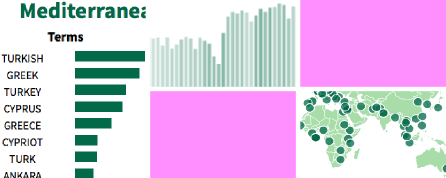
\includegraphics[width=\linewidth]{fig/viz.png}
% \caption{Screenshots of Capsule visualization of US State Department cables.  Left: top words in a topic (manually labeled topic title).  Center-top: events over time (height is volume of messages sent, color is probability of an event occurring).  Center-bottom: topics for an event on <date TODO: cyprus coup?>.  Right-top: cyprus entity topics? TODO.  Right-bottom: entities shown on a map.}
% \label{fig:viz}
% \end{figure}

